\chapter{Especificaci\'on del Proyecto}

\section{Situaci\'on Actual}

\subsection{Antecedentes: El ma\'iz como sustento y la emergencia productiva}

La agricultura representa el 5.6\% del Producto Interno Bruto (PIB) de El Salvador \cite{bcr2023} y sostiene de forma directa a m\'as de dos millones de personas en el sector rural. Para las familias campesinas salvadore\~nas, el ma\'iz (\textit{Zea mays L.}) constituye la base diaria de la alimentaci\'on familiar, con un consumo promedio reportado que supera los 115 kilogramos por persona al a\~no \cite{centa2022}. De acuerdo con registros oficiales del Ministerio de Agricultura y Ganader\'ia \cite{mag2023}, el 82.1\% de los productores nacionales trabajan peque\~nas parcelas familiares menores a dos manzanas (1.4 hect\'areas), bajo un r\'egimen de agricultura de subsistencia dependiente casi por completo del r\'egimen de lluvias estacionales.

En los \'ultimos a\~nos, esta base productiva ha enfrentado una vulnerabilidad creciente frente a anomal\'ias clim\'aticas e incidencia fitosanitaria \cite{mag2023}. En una milpa sometida a estr\'es h\'idrico o t\'ermico, la aparici\'on de enfermedades foliares o plagas no es un fen\'omeno aislado: si una infecci\'on o ataque no se detecta y atiende de forma oportuna, compromete severamente el llenado de grano y la productividad de la cosecha \cite{centa2022}, amenazando de manera directa la seguridad alimentaria y la subsistencia del hogar campesino.

\subsection{Descripci\'on del problema: El diagn\'ostico a ciegas en el surco}

En las parcelas rurales salvadore\~nas no existen microscopios ni laboratorios cercanos. El diagn\'ostico fitosanitario diario descansa por completo en los ojos del agricultor, quien recorre el surco bajo el sol, entre polvo y calor, tratando de interpretar manchas y marchitamientos complejos:
\begin{itemize}
\item \textbf{Tiz\'on foliar (\textit{Exserohilum turcicum}) y mancha gris (\textit{Cercospora zeae-maydis}):} Colonizan la l\'amina verde con lesiones alargadas o rectangulares que secan la hoja y detienen el llenado de la mazorca.
\item \textbf{Gusano cogollero (\textit{Spodoptera frugiperda}):} Mastica los verticilos tiernos y destruye el punto de crecimiento de la planta.
\item \textbf{Necrosis letal del ma\'iz (MLN):} Complejo viral altamente destructivo que marchita la planta de ra\'iz a espiga y anula el 100\% de la cosecha.
\item \textbf{Deficiencias nutricionales de nitr\'ogeno, f\'osforo y potasio (N-P-K):} Provocan clorosis en ``V'', pigmentaciones p\'urpuras y secado marginal que a simple vista se confunden f\'acilmente con hongos o virus.
\end{itemize}

Esta dificultad se agrava ante la marcada limitaci\'on de cobertura en la asistencia t\'ecnica p\'ublica presencial. La relaci\'on entre el personal t\'ecnico extensionista disponible y el n\'umero global de productores agr\'icolas dispersos en la geograf\'ia rural salvadore\~na genera una brecha estructural de atenci\'on, donde una visita agron\'omica especializada suele demorar semanas o no llegar a materializarse durante la ventana cr\'itica de la infecci\'on \cite{centa2022}.

Ante la incertidumbre y el riesgo inminente de p\'erdida de la siembra, el agricultor acude frecuentemente a puntos comerciales de agroservicios. En estos espacios, la falta de diagn\'ostico instrumental propicia recomendaciones emp\'iricas basadas en agroqu\'imicos de amplio espectro para s\'intomas que corresponden a deficiencias nutricionales de suelo. Esta situaci\'on ocasiona p\'erdidas econ\'omicas significativas para el presupuesto familiar al incurrir en gastos fitosanitarios ineficaces, adem\'as de generar impactos ambientales negativos por sobreaplicaci\'on de qu\'imicos y retrasar la atenci\'on correctiva adecuada de pat\'ogenos severos \cite{centa2022}.

\begin{figure}[H]
\centering
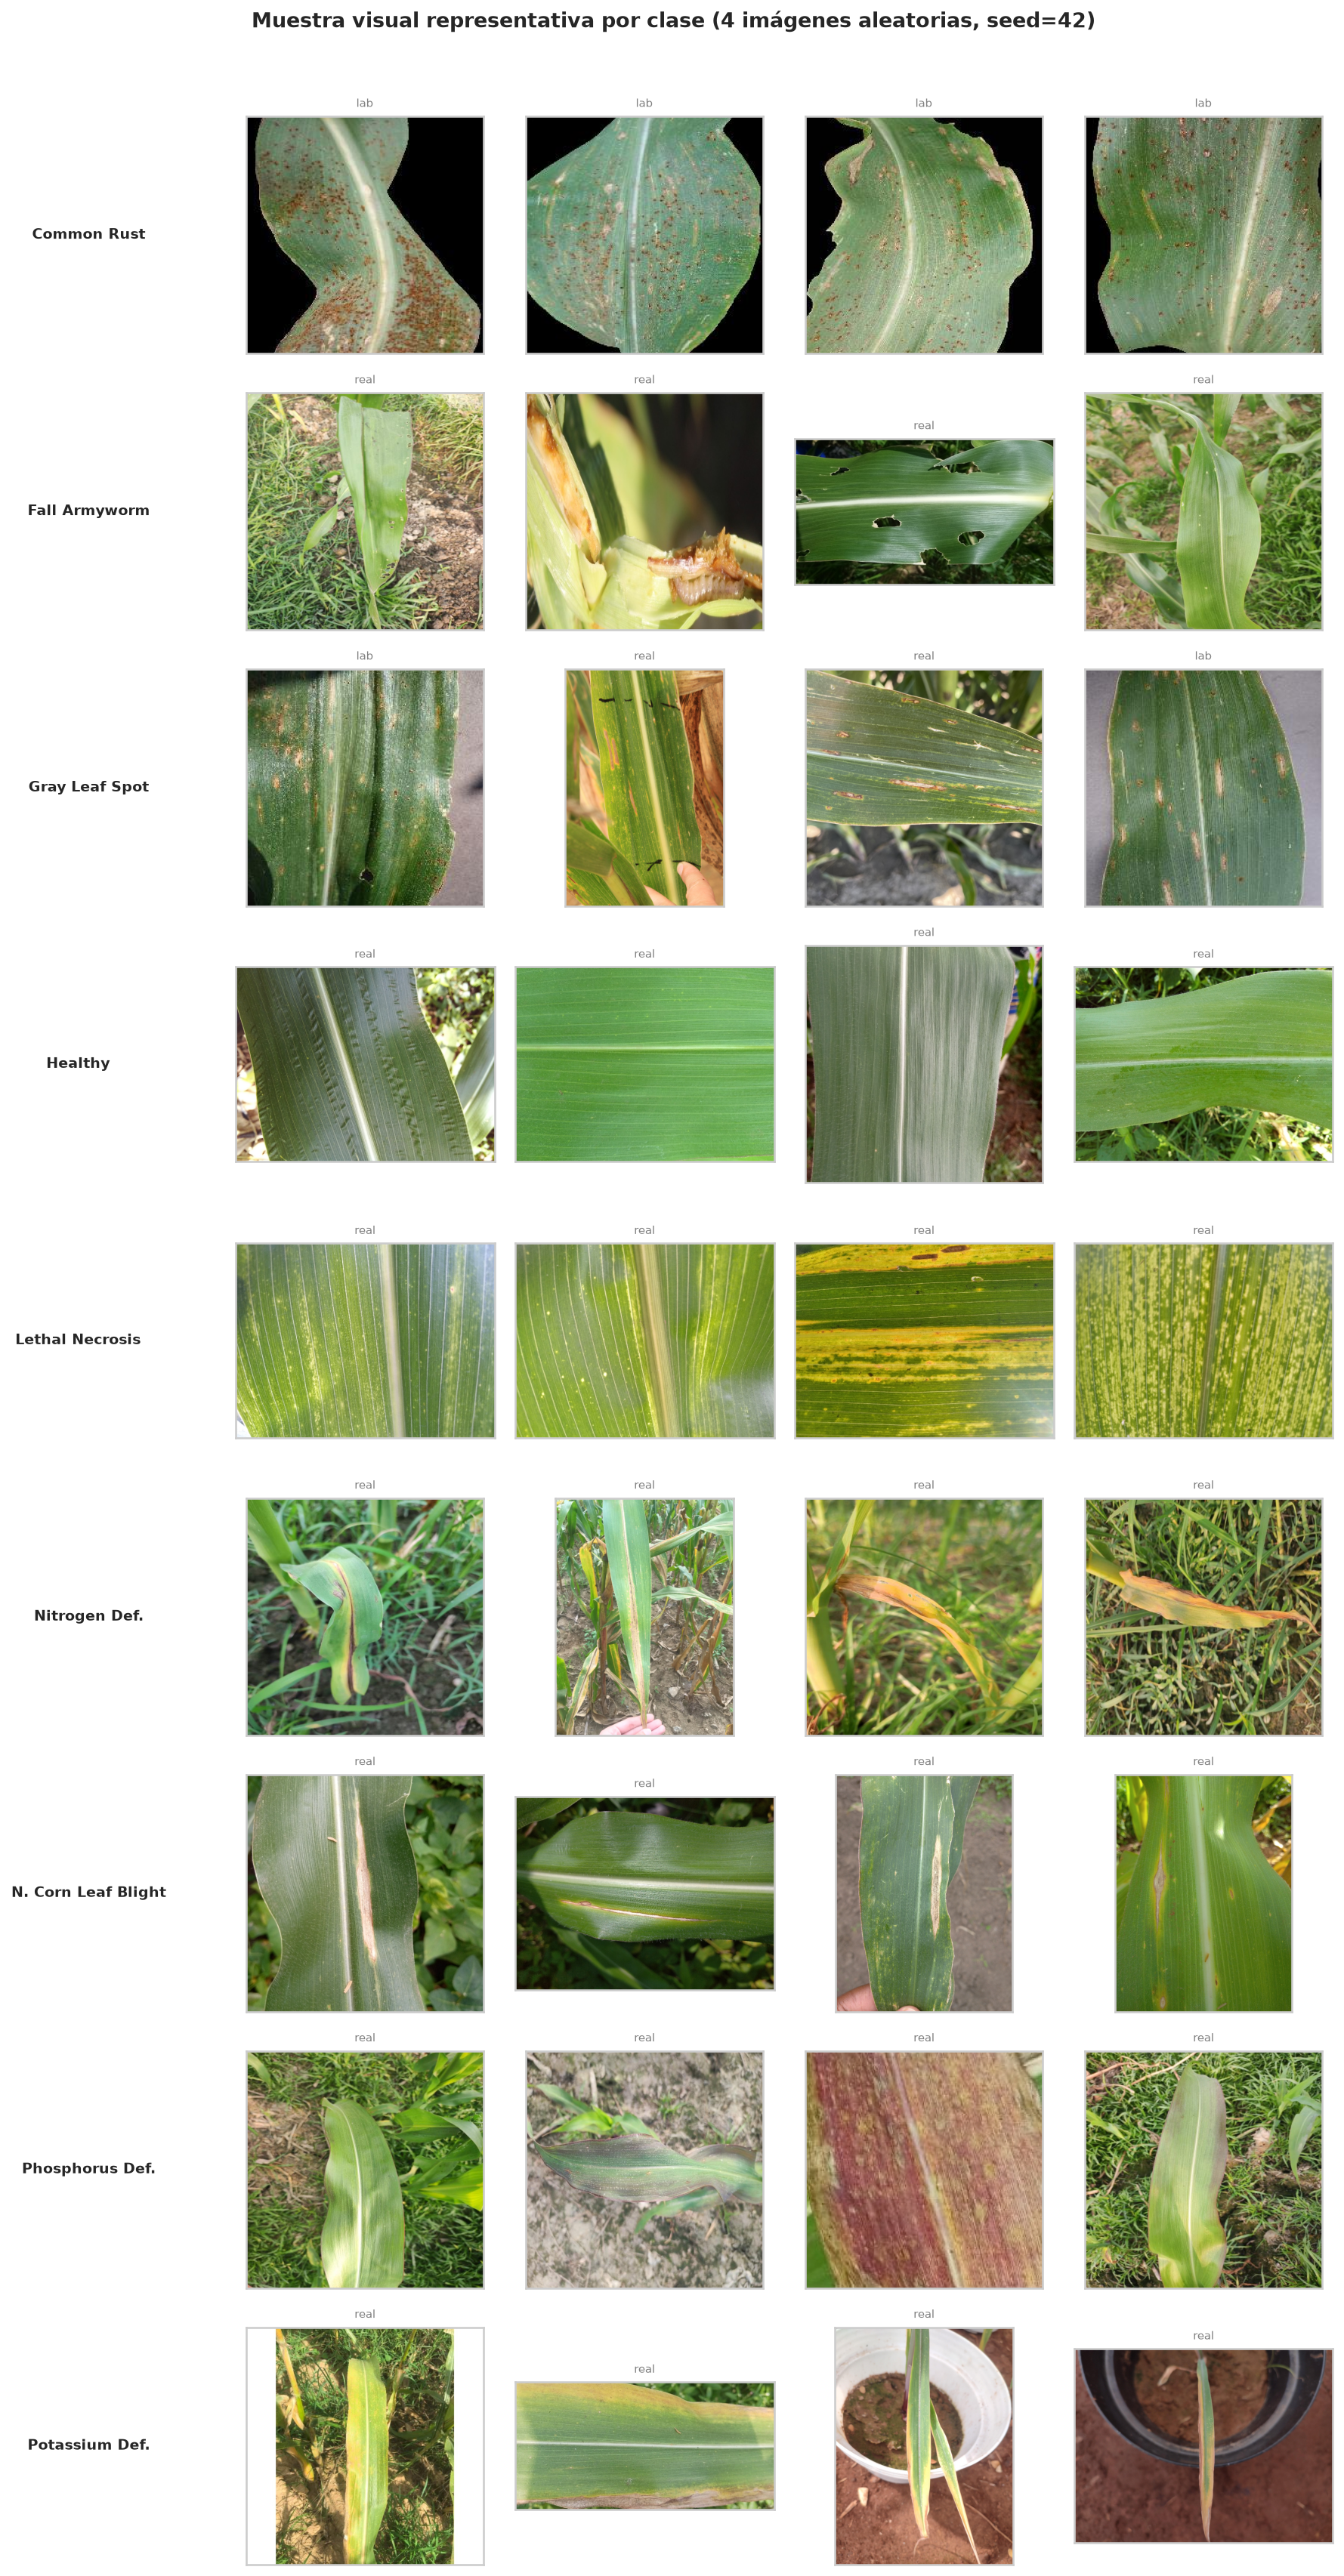
\includegraphics[height=0.74\textheight,keepaspectratio]{images/eda/eda_00_muestra_visual.png}
\caption{Diversidad morfol\'ogica, fondos r\'usticos y heterogeneidad geom\'etrica en las afecciones foliares del ma\'iz.}
\label{fig:eda_samples}
\end{figure}

\subsection{Planteamiento del problema}

A partir de la situaci\'on descrita, se constata que los mecanismos tradicionales de extensi\'on agron\'omica resultan insuficientes para brindar cobertura a los peque\~nos productores de ma\'iz en El Salvador, mientras que las herramientas digitales contempor\'aneas han sido concebidas bajo premisas incompatibles con la realidad rural. En la pr\'actica, las soluciones comerciales de visi\'on artificial presentan tres limitaciones cr\'iticas:

\begin{enumerate}
\item \textbf{Dependencia de conectividad de red:} La mayor parte de las aplicaciones disponibles requieren comunicaci\'on permanente con servidores en la nube para procesar las capturas. En el agro salvadore\~no, donde extensas zonas rurales presentan cobertura celular inestable o nula y los agricultores no disponen de planes continuos de transmisi\'on de datos, esta dependencia anula la utilidad pr\'actica de las herramientas en el propio surco.
\item \textbf{Incompatibilidad con terminales b\'asicos:} Los modelos de aprendizaje profundo convencionales demandan una capacidad de c\'omputo y memoria que excede con creces los recursos de los tel\'efonos inteligentes accesibles para las familias campesinas (dispositivos de gama de entrada con 2 a 4~GB de RAM), provocando bloqueos, latencias intolerables y un r\'apido consumo de bater\'ia.
\item \textbf{Vulnerabilidad ante la variabilidad del entorno real:} Al haber sido entrenados mayoritariamente sobre im\'agenes de laboratorio con fondos neutros e iluminaci\'on homog\'enea, los algoritmos colapsan al exponerse a la milpa, donde la presencia de suelos r\'usticos, sombras irregulares, malezas y contraluz induce clasificaciones err\'oneas emitidas con un alto grado de sobreconfianza.
\end{enumerate}

Frente a este escenario, surge la necesidad de replantear el diagn\'ostico automatizado desde las restricciones materiales del entorno agr\'icola. Una herramienta orientada a cerrar esta brecha debe operar directamente en manos del productor, fundament\'andose en cuatro requerimientos operacionales esenciales:

\begin{itemize}
\item \textbf{Autonom\'ia operativa local:} La capacidad diagn\'ostica debe ejecutarse de forma integral en el propio dispositivo, asegurando disponibilidad inmediata en la parcela sin supeditar su funcionamiento a redes de telecomunicaciones.
\item \textbf{Austeridad y eficiencia computacional:} El procesamiento debe ajustarse estrictamente a las capacidades t\'ecnicas de los tel\'efonos b\'asicos predominantes en las zonas rurales, garantizando tiempos de respuesta cortos y un consumo m\'inimo de energ\'ia.
\item \textbf{Resiliencia y bioseguridad ante la captura:} El sistema debe ser capaz de discriminar la sintomatolog\'ia foliar frente al ruido visual del campo y, de manera primordial, reconocer situaciones de incertidumbre o tomas no v\'alidas para abstenerse de emitir diagn\'osticos infundados que perjudiquen la econom\'ia familiar.
\item \textbf{Traducci\'on agron\'omica orientada a la acci\'on:} El diagn\'ostico visual debe complementarse con una evaluaci\'on comprensible del nivel de da\~no y con alternativas concretas de manejo integrado basadas en bioinsumos accesibles, facilitando una intervenci\'on oportuna y viable para el productor.
\end{itemize}

Con base en estas consideraciones, se formula la problem\'atica central de la investigaci\'on:
\begin{quote}
\centering
\itshape
\textquestiondown En qu\'e medida es factible concebir, desarrollar y evaluar una aplicaci\'on m\'ovil de diagn\'ostico fitosanitario que opere de manera aut\'onoma en tel\'efonos inteligentes de gama baja o media, capaz de discernir patolog\'ias foliares en condiciones reales de campo, gestionar la incertidumbre de la captura y orientar oportunamente al agricultor salvadore\~no en el manejo integrado de su cultivo?
\end{quote}

\subsubsection{Modelo conceptual de caja negra del sistema}

Con el prop\'osito de delimitar anal\'iticamente este problema sin prejuzgar la arquitectura interna que deber\'a investigarse y validarse experimentalmente en los cap\'itulos posteriores, el sistema se conceptualiza mediante el modelo de caja negra (Figura~\ref{fig:caja_negra}). En la ingenier\'ia de sistemas, este enfoque formaliza la relaci\'on entre los est\'imulos y restricciones del entorno problem\'atico (entradas) y los resultados requeridos para mitigar la problem\'atica (salidas), definiendo el n\'ucleo del sistema como el proceso de transformaci\'on tecnol\'ogica que constituye el objeto de estudio de esta investigaci\'on:

\begin{figure}[H]
\centering
\resizebox{0.98\textwidth}{!}{%
\begin{tikzpicture}[
    node distance=1.0cm and 0.9cm,
    header/.style={
        rectangle,
        rounded corners=3pt,
        minimum width=5.2cm,
        minimum height=0.75cm,
        text centered,
        font=\bfseries\small,
        text=white
    },
    card/.style={
        rectangle,
        rounded corners=5pt,
        minimum width=5.3cm,
        text width=4.9cm,
        inner sep=8pt,
        font=\scriptsize,
        draw=gray!35,
        line width=1pt,
        align=left
    },
    arrow/.style={
        -{Latex[length=3.5mm,width=2.5mm]},
        line width=1.8pt,
        draw=gray!70
    }
]

% --- COLUMNA 1: ENTRADA ---
\node[header, fill=blue!75!black] (head_in) {Entradas};
\node[card, fill=blue!3, below=0.15cm of head_in] (box_in) {
  \textbf{Condiciones del Entorno Rural:}
  \begin{itemize}\setlength{\itemsep}{2pt}\setlength{\leftskip}{-10pt}
    \item Fotograf\'ias foliares capturadas por el agricultor en parcelas reales.
    \item Iluminaci\'on solar directa no uniforme, sombras duras y fondos r\'usticos.
    \item Sintomatolog\'ia foliar diversa y estados fenol\'ogicos heterog\'eneos.
  \end{itemize}
  \vspace{0.12cm}
  \textbf{Restricciones Operativas del Problema:}
  \begin{itemize}\setlength{\itemsep}{2pt}\setlength{\leftskip}{-10pt}
    \item Ausencia total de conectividad m\'ovil o internet en el surco.
    \item Tel\'efonos inteligentes b\'asicos con recursos acotados de memoria y procesador.
  \end{itemize}
};

% --- COLUMNA 2: CAJA NEGRA (PROCESO) ---
\node[header, fill=gray!80!black, right=1.4cm of head_in] (head_proc) {Procesos};
\node[card, fill=gray!4, below=0.15cm of head_proc] (box_proc) {
  \textbf{Transformaci\'on Requerida:}
  \begin{itemize}\setlength{\itemsep}{2pt}\setlength{\leftskip}{-10pt}
    \item Procesamiento y an\'alisis visual local en el dispositivo m\'ovil.
    \item Discriminaci\'on de afecciones foliares frente al ruido del entorno.
    \item Evaluaci\'on de confiabilidad y validez de la captura realizada.
    \item Vinculaci\'on de la evidencia \'optica con directrices agron\'omicas.
  \end{itemize}
  \vspace{0.12cm}
  \textbf{Desaf\'io de Ingenier\'ia e Investigaci\'on:}
  \begin{itemize}\setlength{\itemsep}{2pt}\setlength{\leftskip}{-10pt}
    \item \textquestiondown C\'omo lograr sensibilidad diagn\'ostica y resiliencia ante entornos r\'usticos dentro de los l\'imites estrictos de un m\'ovil modesto?
  \end{itemize}
};

% --- COLUMNA 3: SALIDA ESPERADA ---
\node[header, fill=teal!70!black, right=1.4cm of head_proc] (head_out) {Salidas esperadas};
\node[card, fill=teal!3, below=0.15cm of head_out] (box_out) {
  \textbf{Diagn\'ostico y Bioseguridad:}
  \begin{itemize}\setlength{\itemsep}{2pt}\setlength{\leftskip}{-10pt}
    \item Detecci\'on temprana y diferenciada de la afecci\'on foliar evaluada.
    \item Alta sensibilidad en patolog\'ias cr\'iticas para evitar p\'erdidas totales.
    \item Distinci\'on confiable entre plagas, enfermedades y deficiencias nutricionales.
  \end{itemize}
  \vspace{0.12cm}
  \textbf{Decisi\'on Fitosanitaria en Parcela:}
  \begin{itemize}\setlength{\itemsep}{2pt}\setlength{\leftskip}{-10pt}
    \item Alerta preventiva y abstenci\'on ante im\'agenes dudosas («No reconocida»).
    \item Orientaci\'on de severidad y bioinsumos en lenguaje claro y accesible.
    \item Prevenci\'on del gasto infructuoso en agroqu\'imicos inapropiados.
  \end{itemize}
};

% --- FLECHAS DE CONEXIÓN ---
\draw[arrow] (box_in.east) -- (box_proc.west);
\draw[arrow] (box_proc.east) -- (box_out.west);

\end{tikzpicture}%
}
\caption{Modelo conceptual de caja negra para el diagn\'ostico fitosanitario m\'ovil.}
\label{fig:caja_negra}
\end{figure}

Como sintetiza la Figura~\ref{fig:caja_negra}, el modelo de caja negra formaliza la l\'ogica de la investigaci\'on: establece c\'omo las restricciones de campo y los desaf\'ios visuales del cultivo ingresan a un proceso de transformaci\'on m\'ovil concebido para generar diagn\'osticos confiables y decisiones fitosanitarias oportunas para el campesino. A partir de esta delimitaci\'on del problema, se formulan a continuaci\'on los objetivos de la investigaci\'on.

\section{Objetivos}

\subsection{Objetivo General}

Desarrollar, evaluar e implementar un sistema de visi\'on artificial embebido (\textit{Edge AI}) para el diagn\'ostico fitosanitario a partir de im\'agenes de la hoja de ma\'iz en El Salvador, desplegado mediante una aplicaci\'on m\'ovil nativa de operaci\'on completamente desconectada (\textit{offline}), capaz de clasificar afecciones foliares con alta sensibilidad y baja latencia en tel\'efonos inteligentes de gama baja o media.

\subsection{Objetivos Espec\'ificos}

\begin{enumerate}
\item Consolidar, depurar y auditar criptogr\'aficamente un conjunto multimodal de m\'as de 33~000 im\'agenes de la hoja de ma\'iz distribuidas en 9 condiciones agron\'omicas, estableciendo contratos de datos verificables para descartar duplicados y prevenir filtraciones entre particiones.
\item Optimizar arquitecturas convolucionales ligeras preentrenadas mediante b\'usqueda bayesiana de hiperpar\'ametros (Optuna) y algoritmos de poda temprana, maximizando el Macro $F_1$-Score con un uso eficiente del c\'omputo en GPU.
\item Dise\~nar una estrategia de ensamble por votaci\'on suave (\textit{Soft Voting}) que combine modelos con diferentes sesgos inductivos, con el fin de elevar la sensibilidad diagn\'ostica en patolog\'ias cr\'iticas de la hoja de ma\'iz y mitigar el desbalance de clases.
\item Evaluar el desempe\~no del sistema bajo protocolos de validaci\'on cruzada agrupada por procedencia (\textit{SourceGroupedKFold}), cuantificando la disparidad de impacto entre laboratorio y campo real, as\'i como la atribuci\'on espacial mediante t\'ecnicas de explicabilidad y ablaci\'on de fondo.
\item Cuantizar la arquitectura neuronal a enteros de 8 bits (Int8) e integrarla en una aplicaci\'on m\'ovil nativa provista de marco gu\'ia de encuadre y detector de tomas an\'omalas, validando su precisi\'on y fluidez en tel\'efonos inteligentes f\'isicos de gama baja o media.
\item Formular una propuesta estrat\'egica de integraci\'on institucional y pol\'iticas p\'ublicas orientada al Ministerio de Agricultura y Ganader\'ia (MAG) y al CENTA, que facilite la transferencia tecnol\'ogica y el acompa\~namiento t\'ecnico a los peque\~nos productores de ma\'iz.
\end{enumerate}

\section{Alcance y L\'imites del Proyecto}

\subsection{Alcance del Proyecto}

El alcance del presente proyecto comprende la investigaci\'on, dise\~no, desarrollo e implementaci\'on de una soluci\'on integral de diagn\'ostico fitosanitario orientada a los peque\~nos productores de ma\'iz en El Salvador. La soluci\'on se materializa en dos componentes tecnol\'ogicos articulados: la aplicaci\'on m\'ovil nativa para el usuario final y el motor anal\'itico de visi\'on artificial embebida.

\subsubsection{Alcance de la Aplicaci\'on M\'ovil (DoctorMaiz)}
La aplicaci\'on m\'ovil constituye el punto de interacci\'on directa en manos del agricultor y abarca las siguientes capacidades funcionales:
\begin{itemize}
\item \textbf{Inferencia local aut\'onoma (\textit{Offline}):} Ejecuci\'on integral del motor neuronal en el procesador del tel\'efono mediante modelos cuantizados, asegurando diagn\'osticos instant\'aneos en el surco sin requerir conexi\'on a internet ni datos m\'oviles.
\item \textbf{Captura asistida con marco gu\'ia foliar:} Interfaz de c\'amara con ret\'icula visual ergon\'omica que orienta al agricultor a encuadrar la l\'amina de la hoja, reduciendo la captura de fondos distractores (suelo, sombras o maleza) antes de procesar la imagen.
\item \textbf{Detecci\'on preventiva de capturas an\'omalas (Seguridad OOD):} M\'odulo de rechazo ante muestras fuera de dominio capaz de evaluar si la captura no corresponde a una hoja de ma\'iz o presenta incertidumbre excesiva, notificando un estado de «No reconocida» para evitar diagn\'osticos enga\~nosos.
\item \textbf{Diagn\'ostico y valoraci\'on de severidad:} Presentaci\'on de resultados en lenguaje claro y accesible, categorizando la afecci\'on con una escala visual de severidad en tres niveles (leve, moderada y severa) para apoyar la toma de decisiones.
\item \textbf{Cat\'alogo de manejo integrado y bioinsumos:} Gu\'ia fitosanitaria pr\'actica vinculada al diagn\'ostico que ofrece alternativas de bioinsumos y manejo cultural de bajo costo, previniendo gastos perjudiciales en agroqu\'imicos inapropiados.
\item \textbf{Historial y georreferenciaci\'on de muestreos:} Registro local persistente de cada evaluaci\'on (fecha, diagn\'ostico, severidad y ubicaci\'on GPS) para que el agricultor monitoree la evoluci\'on de sus parcelas a lo largo del ciclo agr\'icola.
\item \textbf{Contribuci\'on comunitaria y sincronizaci\'on voluntaria:} M\'odulo opcional que permite almacenar im\'agenes validadas localmente para compartirlas cuando se cuente con conectividad, contribuyendo al monitoreo fitosanitario colectivo.
\end{itemize}

\subsubsection{Alcance del Componente de Inteligencia Artificial Embebida}
El n\'ucleo de aprendizaje profundo embebido abarca:
\begin{itemize}
\item \textbf{Cobertura taxon\'omica de 9 clases en hoja de ma\'iz:} Clasificaci\'on supervisada de signos y s\'intomas foliares, cubriendo enfermedades causadas por hongos (tiz\'on foliar, mancha gris y roya com\'un), virosis cr\'itica (necrosis letal del ma\'iz), plagas directas (gusano cogollero), deficiencias nutricionales de suelo (nitr\'ogeno, f\'osforo y potasio) y l\'amina foliar sana.
\item \textbf{Optimizaci\'on bayesiana, ensamble y cuantizaci\'on Int8:} B\'usqueda automatizada de hiperpar\'ametros (Optuna con poda temprana), combinaci\'on estrat\'egica por votaci\'on suave (\textit{Soft Voting}) y cuantizaci\'on a 8 bits exportada en formato TensorFlow Lite mediante litert-torch, optimizada para inferencia ultrarr\'apida ($\le 100$~ms) en procesadores m\'oviles.
\item \textbf{Auditor\'ia de sesgos y generalizaci\'on:} Protocolo de evaluaci\'on cruzada agrupada por procedencia (\textit{SourceGroupedKFold}) y pruebas de ablaci\'on espacial de fondo para auditar y neutralizar el fen\'omeno de atajos visuales (\textit{Clever Hans effect}).
\end{itemize}

\subsection{L\'imites y Fronteras del Proyecto}

Con el fin de delimitar con precisi\'on la cobertura de la investigaci\'on, se definen los siguientes l\'imites operacionales:
\begin{itemize}
\item \textbf{L\'imite biol\'ogico y sintom\'atico:} El sistema se restringe exclusivamente al an\'alisis de afecciones visibles en la l\'amina foliar del ma\'iz. Quedan fuera del alcance patolog\'ias radiculares, afecciones del tallo interno sin expresi\'on foliar y el monitoreo de plagas subterr\'aneas.
\item \textbf{L\'imite de plataforma y compatibilidad de hardware:} La soluci\'on m\'ovil se enfoca en dispositivos con sistema operativo Android 7.0 o superior con arquitectura de procesador ARM (v7 o v8), c\'amara trasera con enfoque autom\'atico y al menos 2~GB de memoria RAM. No se contempla desarrollo nativo para iOS ni para tel\'efonos sin capacidades inteligentes.
\item \textbf{L\'imite de infraestructura y red:} La aplicaci\'on est\'a dise\~nada para operar desconectada; no existe dependencia de servicios en la nube para emitir el diagn\'ostico, ni se incluye sincronizaci\'on transaccional en tiempo real entre m\'ultiples terminales.
\item \textbf{L\'imite legal y de diagn\'ostico fitopatol\'ogico:} La herramienta constituye un asistente t\'ecnico de orientaci\'on y apoyo agron\'omico para el productor. En ning\'un caso reemplaza los ensayos fitopatol\'ogicos de laboratorio (cultivos, aislamiento microbiano o pruebas PCR), ni sustituye los dict\'amenes oficiales de cuarentena o certificaci\'on fitosanitaria del Ministerio de Agricultura y Ganader\'ia.
\end{itemize}

\section{Hip\'otesis}

\subsection{Hip\'otesis General}
El dise\~no propone un sistema de visi\'on artificial embebido en una aplicaci\'on m\'ovil nativa, con captura asistida y operaci\'on completamente desconectada, capaz de clasificar nueve condiciones agron\'omicas de la hoja de ma\'iz en tel\'efonos inteligentes de gama baja o media del sector rural salvadore\~no. Se considera alcanzado el objetivo general si se cumplen los criterios de la Tabla~\ref{tab:criterios_exito}.

\subsection{Criterios de \'Exito Espec\'ificos}
Los criterios siguientes son las condiciones que el sistema debe cumplir para considerar alcanzado cada objetivo. Se verifican en el cap\'itulo de resultados y se agrupan en cuatro temas.

\begin{table}[H]
\caption{Criterios de \'exito del proyecto, agrupados por tema}
\label{tab:criterios_exito}
\centering
\small
\begin{singlespace}
\begin{tabularx}{\textwidth}{>{\raggedright\arraybackslash}p{3.4cm}>{\raggedright\arraybackslash}X>{\raggedright\arraybackslash}p{3.2cm}}
\toprule
\textbf{Tema} & \textbf{Criterio y umbral} & \textbf{M\'etrica} \\
\midrule
Ahorro de entrenamiento & Reducir en al menos 40\% las horas de GPU frente a una b\'usqueda sin poda temprana. & Horas de GPU por corrida \\
Rendimiento del modelo & Alcanzar Macro $F_1 \ge 0.85$ en la partici\'on de prueba retenida, con recall de la necrosis letal (MLN) $\ge 95\%$. & Macro $F_1$, recall por clase \\
Capacidades del diagn\'ostico & Mantener un \textit{Disparate Impact Ratio} $\ge 0.80$ entre laboratorio y campo real, y rechazar fuera de dominio las im\'agenes que no son hojas de ma\'iz. & DIR, umbral OOD \\
Soluci\'on integral & Modelo Int8 menor a 5~MB, inferencia en menos de 100~ms en un tel\'efono de gama media y funcionamiento sin conexi\'on. & Tama\~no, latencia \\
\bottomrule
\end{tabularx}
\end{singlespace}
\end{table}

\section{Justificaci\'on}

\subsection{Justificaci\'on T\'ecnica y Metodol\'ogica}
La presente investigaci\'on se justifica t\'ecnicamente al trasladar el procesamiento de aprendizaje profundo desde arquitecturas dependientes de servidores en la nube hacia el borde del dispositivo m\'ovil (\textit{Edge AI}). En la literatura especializada de visi\'on por computadora aplicada a la agricultura, predomina el entrenamiento de modelos convolucionales de alta complejidad evaluados sobre particiones aleatorias convencionales, las cuales frecuentemente sufren de fuga de informaci\'on e introducen atajos visuales ligados a fondos controlados \cite{ahmad2023a}. El presente proyecto aborda esta limitaci\'on mediante una metodolog\'ia rigurosa basada en auditor\'ia de duplicados a nivel de p\'ixel, esquemas de validaci\'on cruzada agrupada por procedencia y t\'ecnicas de cuantizaci\'on sim\'etrica a enteros de 8 bits (\textit{Int8}) que reducen dr\'asticamente la demanda computacional sin comprometer la sensibilidad diagn\'ostica \cite{howard2017,tan2019}. Asimismo, integra salvaguardas operacionales como el filtrado de muestras fuera de dominio (\textit{OOD}) \cite{lee2018} y mecanismos de explicabilidad visual mediante mapas de activaci\'on \cite{selvaraju2017}, con el fin de que las predicciones se apoyen en caracter\'isticas de la l\'amina foliar; la verificaci\'on de este objetivo se presenta en el cap\'itulo de resultados.

\subsection{Justificaci\'on Econ\'omica}
Para las peque\~nas familias productoras de ma\'iz en El Salvador, el margen de rentabilidad agr\'icola por ciclo es sumamente reducido y altamente vulnerable a sobrecostos imprevistos \cite{mag2023}. Un diagn\'ostico fitosanitario err\'oneo conduce a la compra e intoxicaci\'on del cultivo con agroqu\'imicos comerciales inadecuados, mermando el escaso capital de trabajo disponible. Proveer una aplicaci\'on m\'ovil de uso aut\'onomo, gratuito y local en el propio tel\'efono inteligente del agricultor permite orientar de manera precisa la intervenci\'on fitosanitaria, evitando gastos innecesarios en plaguicidas ante s\'intomas provocados por deficiencias nutricionales y facilitando una acci\'on temprana contra plagas destructivas como el gusano cogollero (\textit{Spodoptera frugiperda}) antes de que comprometan el rendimiento econ\'omico de la milpa \cite{centa2022}.

\subsection{Justificaci\'on Social y Ambiental}
Desde la perspectiva social, la implementaci\'on de \textit{DoctorMaiz} contribuye a reducir la brecha tecnol\'ogica en comunidades rurales con acceso limitado o nulo a servicios presenciales de extensi\'on agron\'omica \cite{centa2022}. Al transformar un tel\'efono celular com\'un de gama baja o media en un asistente de orientaci\'on fitopatol\'ogica disponible en el surco, se empodera al productor con informaci\'on t\'ecnica comprensible y oportuna. En la dimensi\'on ambiental, un diagn\'ostico certero fomenta el manejo integrado de plagas, desincentivando la aplicaci\'on indiscriminada de pesticidas sint\'eticos y coadyuvando a la protecci\'on de los recursos h\'idricos y la salud de las comunidades rurales.

\subsection{Justificaci\'on Acad\'emica e Institucional}
En el \'ambito acad\'emico e institucional, este proyecto representa una contribuci\'on significativa para la Escuela de Ingenier\'ia de Sistemas Inform\'aticos de la Universidad de El Salvador (UES), al articular la investigaci\'on aplicada en inteligencia artificial embebida con la soluci\'on de problemas prioritarios del desarrollo agropecuario nacional. La investigaci\'on sienta un precedente metodol\'ogico formal para el desarrollo, evaluaci\'on imparcial y despliegue de sistemas de visi\'on artificial adaptados a contextos de recursos computacionales y conectividad restringidos en Centroam\'erica.

\section{Cronograma de Actividades}

La planificaci\'on y ejecuci\'on del proyecto se estructur\'o bajo las fases de la metodolog\'ia \textit{CRISP-DM} (\textit{Cross-Industry Standard Process for Data Mining}), adaptada a los requerimientos de desarrollo de aprendizaje profundo embebido (\textit{Edge AI}) e ingenier\'ia de software m\'ovil. El cronograma abarc\'o un periodo de 28 semanas calendario, iniciando formalmente el 14 de abril de 2026 y culminando con el hito de presentaci\'on y defensa final el 29 de octubre de 2026.

La Figura~\ref{fig:gantt_cronograma} ilustra el diagrama temporal de Gantt y la concurrencia operativa de las fases a lo largo de las 28 semanas del ciclo, mientras que la Tabla~\ref{tab:cronograma} detalla la distribuci\'on de actividades, duraci\'on, horas estimadas y entregables t\'ecnicos por cada etapa.

\begin{figure}[H]
\centering
\caption{Diagrama de Gantt de ejecuci\'on temporal del proyecto (Metodolog\'ia CRISP-DM)}
\label{fig:gantt_cronograma}
\resizebox{\textwidth}{!}{%
\begin{ganttchart}[
    vgrid={draw=black!15, line width=.4pt},
    hgrid={draw=black!10, line width=.4pt},
    canvas/.append style={draw=black!30, line width=.75pt},
    title/.style={draw=black!30, fill=black!5},
    title label font=\bfseries\small,
    bar/.append style={line width=.5pt, rounded corners=2pt},
    bar height=.6,
    bar label font=\small,
    milestone/.append style={line width=.5pt},
    milestone height=.65,
    milestone label font=\bfseries\small,
    x unit=0.52cm,
    y unit chart=0.75cm,
    y unit title=0.6cm
]{1}{28}
\gantttitle{Abr}{3} \gantttitle{May}{4} \gantttitle{Jun}{4} \gantttitle{Jul}{5} \gantttitle{Ago}{4} \gantttitle{Sep}{4} \gantttitle{Oct}{4} \\
\gantttitle{S1--3}{3} \gantttitle{S4--7}{4} \gantttitle{S8--11}{4} \gantttitle{S12--16}{5} \gantttitle{S17--20}{4} \gantttitle{S21--24}{4} \gantttitle{S25--28}{4} \\
\ganttbar[bar/.append style={fill=blue!65!black, draw=blue!90!black}]{Fase 1: Negocio y Datos}{1}{4} \\
\ganttbar[bar/.append style={fill=cyan!65!black, draw=cyan!90!black}]{Fase 2: Preparaci\'on de Datos}{5}{8} \\
\ganttbar[bar/.append style={fill=teal!70!black, draw=teal!90!black}]{Fase 3: Modelado y Optuna}{9}{14} \\
\ganttbar[bar/.append style={fill=orange!75!black, draw=orange!90!black}]{Fase 4: Evaluaci\'on y Sesgos}{15}{18} \\
\ganttbar[bar/.append style={fill=green!60!black, draw=green!80!black}]{Fase 5: Edge AI y App M\'ovil}{19}{24} \\
\ganttbar[bar/.append style={fill=purple!65!black, draw=purple!90!black}]{Fase 6: Pruebas y Memoria}{25}{28} \\
\ganttmilestone[milestone/.append style={fill=red!80!black, draw=red!90!black}]{Hito: Defensa Final (29/10)}{28}
\end{ganttchart}%
}
\end{figure}

\begin{table}[H]
\caption{Cronograma consolidado de actividades y fases del proyecto (CRISP-DM)}
\label{tab:cronograma}
\centering
\small
\begin{singlespace}
\begin{tabularx}{\textwidth}{p{4.3cm}ccccX}
\toprule
\textbf{Fase / Actividad Operativa} & \textbf{Inicio} & \textbf{Fin} & \textbf{Semanas} & \textbf{Horas} & \textbf{Entregable Principal} \\
\midrule
\textbf{Fase 1: Comprensi\'on del Negocio y Datos} & 14/04/26 & 12/05/26 & 4 & 40 h & Requisitos fitosanitarios y corpus consolidado ($>$33K im\'agenes). \\
\textbf{Fase 2: Preparaci\'on de Datos} & 12/05/26 & 09/06/26 & 4 & 40 h & Auditor\'ia criptogr\'afica de duplicados, balanceo y data augmentation. \\
\textbf{Fase 3: Modelado Algor\'itmico} & 09/06/26 & 21/07/26 & 6 & 60 h & Transfer learning en arquitecturas ligeras y optimizaci\'on con Optuna. \\
\textbf{Fase 4: Evaluaci\'on y Auditor\'ia de Sesgos} & 21/07/26 & 18/08/26 & 4 & 40 h & Ensamble Soft Voting, evaluaci\'on ciega de campo y an\'alisis XAI (Grad-CAM). \\
\textbf{Fase 5: Optimizaci\'on Edge y App M\'ovil} & 18/08/26 & 29/09/26 & 6 & 60 h & Modelo Int8 (3.56~MB), detector OOD y app DoctorMaiz (React Native/Expo). \\
\textbf{Fase 6: Pruebas Finales y Memoria} & 29/09/26 & 29/10/26 & 4 & 40 h & Evaluaci\'on f\'isica en Motorola edge 40 neo, memoria t\'ecnica y defensa final. \\
\midrule
\textbf{Hito Final: Defensa de Proyecto} & \multicolumn{2}{c}{\textbf{29 de octubre de 2026}} & \textbf{28 sem} & \textbf{280 h} & \textbf{Sistema DoctorMaiz liberado} \\
\bottomrule
\end{tabularx}
\end{singlespace}
\end{table}

\section{Presupuesto Global Estimado}

El presupuesto del desarrollo y evaluaci\'on de la soluci\'on anal\'itica y embebida abarc\'o dos categor\'ias esenciales: recurso humano especializado e infraestructura de c\'omputo acelerado en la nube (Tablas~\ref{tab:presupuesto_rh} a~\ref{tab:presupuesto_resumen}). Las horas de GPU se tomaron de los registros de ejecuci\'on del repositorio; el resto de rubros son proyecciones.

\begin{table}[H]
\caption{Presupuesto proyectado: C\'alculo del salario base por rol (280 horas)}
\label{tab:presupuesto_rh}
\centering
\small
\begin{singlespace}
\begin{tabularx}{\textwidth}{>{\raggedright\arraybackslash}X>{\centering\arraybackslash}p{2.6cm}>{\centering\arraybackslash}p{2.6cm}>{\centering\arraybackslash}p{2.6cm}>{\centering\arraybackslash}p{2.6cm}}
\toprule
\textbf{Rol Profesional} & \textbf{Salario mensual de referencia} & \textbf{Meses equivalentes (280 h)} & \textbf{Salario base (USD)} \\
\midrule
Ingeniero de Datos / MLOps & \$1,500.00 & 1.6154 & \$2,423.08 \\
Investigador de Deep Learning & \$1,350.00 & 1.6154 & \$2,180.77 \\
Desarrollador M\'ovil Edge AI & \$1,250.00 & 1.6154 & \$2,019.23 \\
\midrule
\textbf{Total salario base} & \textbf{\$4,100.00} & — & \textbf{\$6,623.08} \\
\bottomrule
\end{tabularx}
\end{singlespace}
\end{table}

\begin{table}[H]
\caption{Presupuesto proyectado: Cargas y prestaciones patronales sobre el salario base}
\label{tab:presupuesto_cargas}
\centering
\small
\begin{singlespace}
\begin{tabularx}{\textwidth}{>{\raggedright\arraybackslash}X>{\centering\arraybackslash}p{1.75cm}>{\centering\arraybackslash}p{1.75cm}>{\centering\arraybackslash}p{1.75cm}>{\centering\arraybackslash}p{2.0cm}>{\centering\arraybackslash}p{1.75cm}>{\centering\arraybackslash}p{2.0cm}}
\toprule
\textbf{Rol Profesional} & \textbf{ISSS 7.5\%} & \textbf{AFP 7.75\%} & \textbf{INSAFORP 1\%} & \textbf{Aguinaldo y vacaciones} & \textbf{Total cargas} & \textbf{Costo total} \\
\midrule
Ingeniero de Datos / MLOps & \$121.15 & \$187.79 & \$24.23 & \$201.92 & \$535.09 & \$2,958.17 \\
Investigador de Deep Learning & \$121.15 & \$169.01 & \$21.81 & \$181.73 & \$493.70 & \$2,674.47 \\
Desarrollador M\'ovil Edge AI & \$121.15 & \$156.49 & \$20.19 & \$168.27 & \$466.10 & \$2,485.33 \\
\midrule
\textbf{Total Recurso Humano} & \textbf{\$363.45} & \textbf{\$513.29} & \textbf{\$66.23} & \textbf{\$551.92} & \textbf{\$1,494.89} & \textbf{\$8,117.97} \\
\bottomrule
\end{tabularx}
\end{singlespace}
\end{table}

Los salarios mensuales corresponden al punto medio de la escala de referencia del sector p\'ublico salvadore\~no para Gobierno Central y Ministerios, aplicada a perfiles equivalentes: Ingeniero de Datos / MLOps (rango de \$1,200 a \$1,800, equivalente a Especialista de Base de Datos o Analista de Sistemas), Investigador de Deep Learning (rango de \$1,100 a \$1,600, equivalente a Especialista en An\'alisis de Datos) y Desarrollador M\'ovil (rango de \$1,000 a \$1,500, equivalente a Analista Programador). La Tabla~\ref{tab:presupuesto_rh} calcula el salario base por rol y la Tabla~\ref{tab:presupuesto_cargas} desglosa las cargas patronales y el costo total. El costo se estima solo por las horas efectivas de trabajo. Cada integrante trabaja de lunes a viernes, menos de 2 horas diarias; para la estimaci\'on se usan 2 horas diarias como cota superior, es decir 10 horas semanales, lo que suma 280 horas en las 28 semanas del cronograma (Tabla~\ref{tab:cronograma}). Equivale a 1.62 meses de una jornada de 40 horas, por lo que el salario mensual de referencia se prorrateó por esa proporci\'on. Las cargas consideran: cuota patronal al ISSS de 7.5\% sobre un salario base m\'aximo de \$1,000.00 mensual; cuota patronal a la AFP de 7.75\%; contribuci\'on al INSAFORP de 1\%; y aguinaldo y vacaciones de ley prorrateados.

\begin{table}[H]
\caption{Presupuesto: Infraestructura Cloud y Licencias}
\label{tab:presupuesto_hw}
\centering
\small
\begin{singlespace}
\begin{tabularx}{\textwidth}{>{\raggedright\arraybackslash}p{3.8cm}>{\raggedright\arraybackslash}X>{\raggedright\arraybackslash}p{4.0cm}>{\raggedleft\arraybackslash}p{2.0cm}}
\toprule
\textbf{Rubro} & \textbf{Detalle T\'ecnico} & \textbf{M\'etrica / Cantidad} & \textbf{Subtotal} \\
\midrule
Instancias GPU Modal & NVIDIA A10G (24 GB VRAM) & 15.85 horas medidas $\times$ \$1.10/h & \$17.44 \\
Almacenamiento Cloud & Cloud Volumes y respaldos de pesos & 100 GB $\times$ 6 meses & \$30.00 \\
Licenciamiento software & PyTorch, Expo, React Native, Optuna & Licencias Open Source / MIT & \$0.00 \\
\midrule
\textbf{Total Infraestructura Cloud y Licencias} & — & — & \textbf{\$47.44} \\
\bottomrule
\end{tabularx}
\end{singlespace}
\end{table}

\begin{table}[H]
\caption{Resumen presupuestario global de la investigaci\'on}
\label{tab:presupuesto_resumen}
\centering
\small
\begin{singlespace}
\begin{tabular}{lcc}
\toprule
\textbf{Rubro de Inversi\'on} & \textbf{Monto Total (USD)} & \textbf{Porcentaje (\%)} \\
\midrule
Recursos Humanos de Investigaci\'on & \$8,117.97 & 99.42\% \\
Servicios de c\'omputo en la nube (GPU/Storage) & \$47.44 & 0.58\% \\
\midrule
\textbf{Total General} & \textbf{\$8,165.41} & \textbf{100.00\%} \\
\bottomrule
\end{tabular}
\end{singlespace}
\end{table}

La ejecuci\'on financiera demuestra que, gracias al aprovechamiento de tecnolog\'ias de c\'odigo abierto y la utilizaci\'on estrat\'egica de cl\'usteres serverless con parada autom\'atica, el costo directo de infraestructura computacional se mantuvo en valores extraordinariamente accesibles (\$47.44 USD, de los cuales \$17.44 corresponden a las 15.85 horas de GPU medidas y \$30.00 al almacenamiento), ratificando la viabilidad econ\'omica de proyectos de investigaci\'on en inteligencia artificial de alto impacto desarrollados en universidades p\'ublicas.
